% Author: Giulio Stramondo, Mail: giuliostramondo[at]gmail.com
\documentclass{standalone}
\usepackage{tikz}
\usetikzlibrary{positioning,arrows,patterns}
\begin{document}
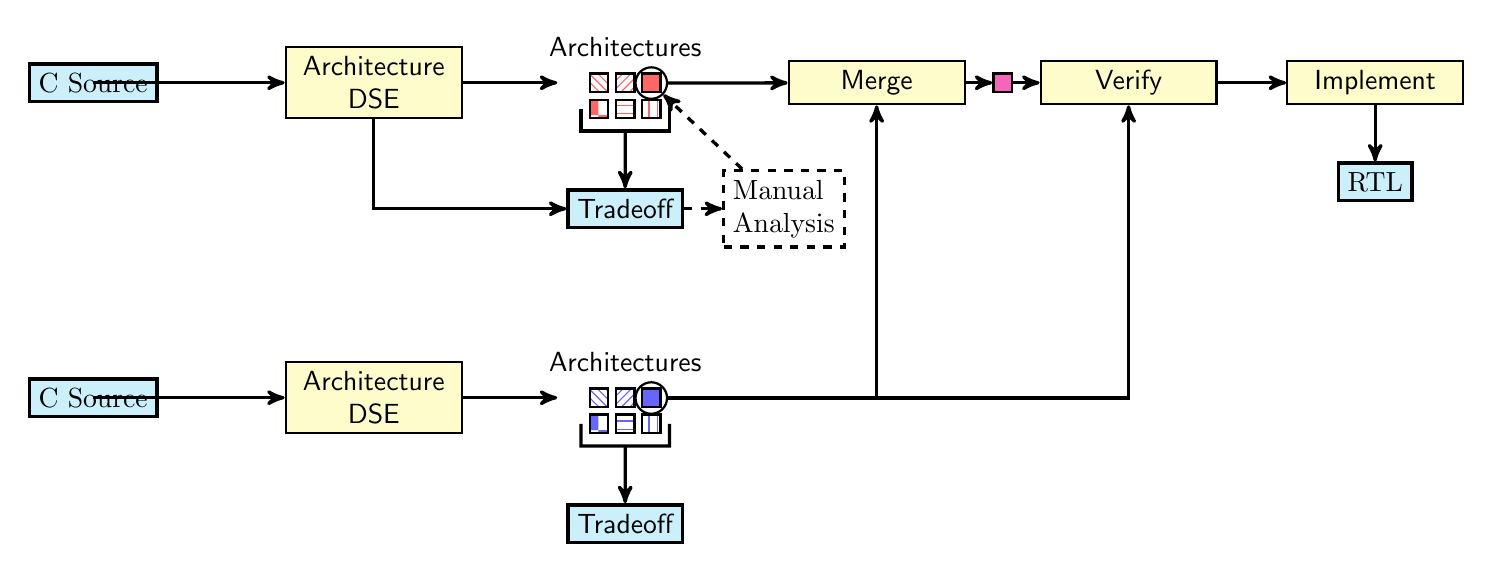
\begin{tikzpicture}[
    archr/.style={rectangle,thick,draw,fill=red!60,anchor=north,
		minimum width=0.2cm},
    archb/.style={rectangle,thick,draw,fill=blue!60,anchor=north,
		minimum width=0.2cm},
    archm/.style={rectangle,thick,draw,fill=magenta!60,anchor=north,
		minimum width=0.2cm},
    select/.style={circle,thick,draw,anchor=north,
		minimum width=0.4cm},
% Event style
    event/.style={rectangle,thick,draw,fill=yellow!20,text width=2cm,
		text centered,font=\sffamily,anchor=north},
%  For compatability with PGF CVS add the absolute option:
   absolute
    ]
%%% Draw system flow diagram
   \begin{scope}[xshift=-7.5cm,yshift=-5cm,very thick,
		node distance=1.6cm,on grid,>=stealth',
		block/.style={rectangle,draw,fill=cyan!20}]
       \node [block] (s1) 	at (0,0)	{C Source};
       \node [event] (step1a) [right=of s1.east] {Architecture DSE};
       \node [archr,pattern=north west lines, pattern color =red!60] (arch1) [right=of step1a.east] {};
       \node [archr,pattern=north east lines, pattern color =red!60] (arch2) [right=of arch1,right=2mm] {};
       \node [archr] (arch3) [left=of arch2,right=2mm] {};
       \node [archr,pattern=horizontal lines, pattern color =red!60] (arch4) [below=of arch2,below=2mm] {};
       \node [archr,pattern=checkerboard, pattern color =red!60] (arch5) [left=of arch4,left=2mm] {};
       \node [archr,pattern=vertical lines, pattern color =red!60] (arch6) [left=of arch4,right=2mm] {};
       \node [] (archlabel) [above=of arch2,above=2mm,font=\sffamily] {Architectures};
       \draw ([xshift=-1mm]arch5.west)  -- ++ (0pt,-8pt) -- ++ (32pt,-0pt) coordinate[xshift=-16pt] (l){} |- ([xshift=1mm]arch6.east);
       \node [block] (analysis) [below=of arch2,font=\sffamily]	{Tradeoff};

       \node [rectangle,draw,dashed,text width=1.3cm, minimum width=0.4cm] (manAnalysis) [right=of analysis,right=35pt]{Manual Analysis};
       \draw[->] (l) -- (analysis);
       \draw[->,dashed] (analysis) -- (manAnalysis);

       \draw[->] (step1a) |- (analysis);
       \draw[->] (step1a) -- ([xshift=-4mm]arch1.west);
       \node [block] (s2)	at (0,-4)   {C Source} ;
       \node [event] (step1b) [right=of s2.east] {Architecture DSE};
       \node [archb,pattern=north west lines, pattern color =blue!60] (arch11) [right=of step1b.east] {};
       \node [archb,pattern=north east lines, pattern color =blue!60] (arch12) [right=of arch11,right=2mm] {};
       \node [archb] (arch13) [left=of arch12,right=2mm] {};
       \node [archb,pattern=horizontal lines, pattern color =blue!60] (arch14) [below=of arch12,below=2mm] {};
       \node [archb,pattern=checkerboard, pattern color =blue!60] (arch15) [left=of arch14,left=2mm] {};
       \node [archb,pattern=vertical lines, pattern color =blue!60] (arch16) [left=of arch14,right=2mm] {};
       \node [] (archlabel1) [above=of arch12,above=2mm,font=\sffamily] {Architectures};
       \draw ([xshift=-1mm]arch15.west)  -- ++ (0pt,-8pt) -- ++ (32pt,-0pt) coordinate[xshift=-16pt] (l1){} -- ([xshift=1mm]arch16.east);
       \node [block] (analysis1) [below=of arch12,font=\sffamily]	{Tradeoff};
       \draw[->] (l1) -- (analysis1);
       \draw[->]  (s1)  |- (step1a);
       \draw[->] (step1b) -- ([xshift=-4mm]arch11.west);
       \draw[->]  (s2)  |- (step1b);
       \node[event] (merge) [right=of arch3.east] {Merge};
       \node[select] (sel1) at ([yshift=2.1mm]arch3.center){};
       \draw[->,dashed] (manAnalysis) -- (sel1);
       \draw[->]  (sel1)  -- (merge);
       \node[select] (sel2) at ([yshift=2.1mm]arch13.center){};
       \draw[->]  (sel2)  -| (merge);
       \node [archm] (archmer) [right=of merge ] {};
       \draw[->]  (merge)  -- (archmer);
       \node[event] (verify) [right=of archmer]{Verify};
       \draw[->]  (archmer) -- (verify);
       \draw[->]  (sel2) -| (verify);
       \node[event] (implement) [right=of verify, right=20mm]{Implement};
       \draw[->]  (verify) -- (implement);
       \node[block] (rtl) [below=of implement, below=10mm]{RTL};
       \draw[->]  (implement) -- (rtl);

   \end{scope}
\end{tikzpicture}
\end{document}

